\section{Dynamic Programming for Joint Speed Optimization}
\label{sec:algorithm}

\begin{figure}[]
  \centering
   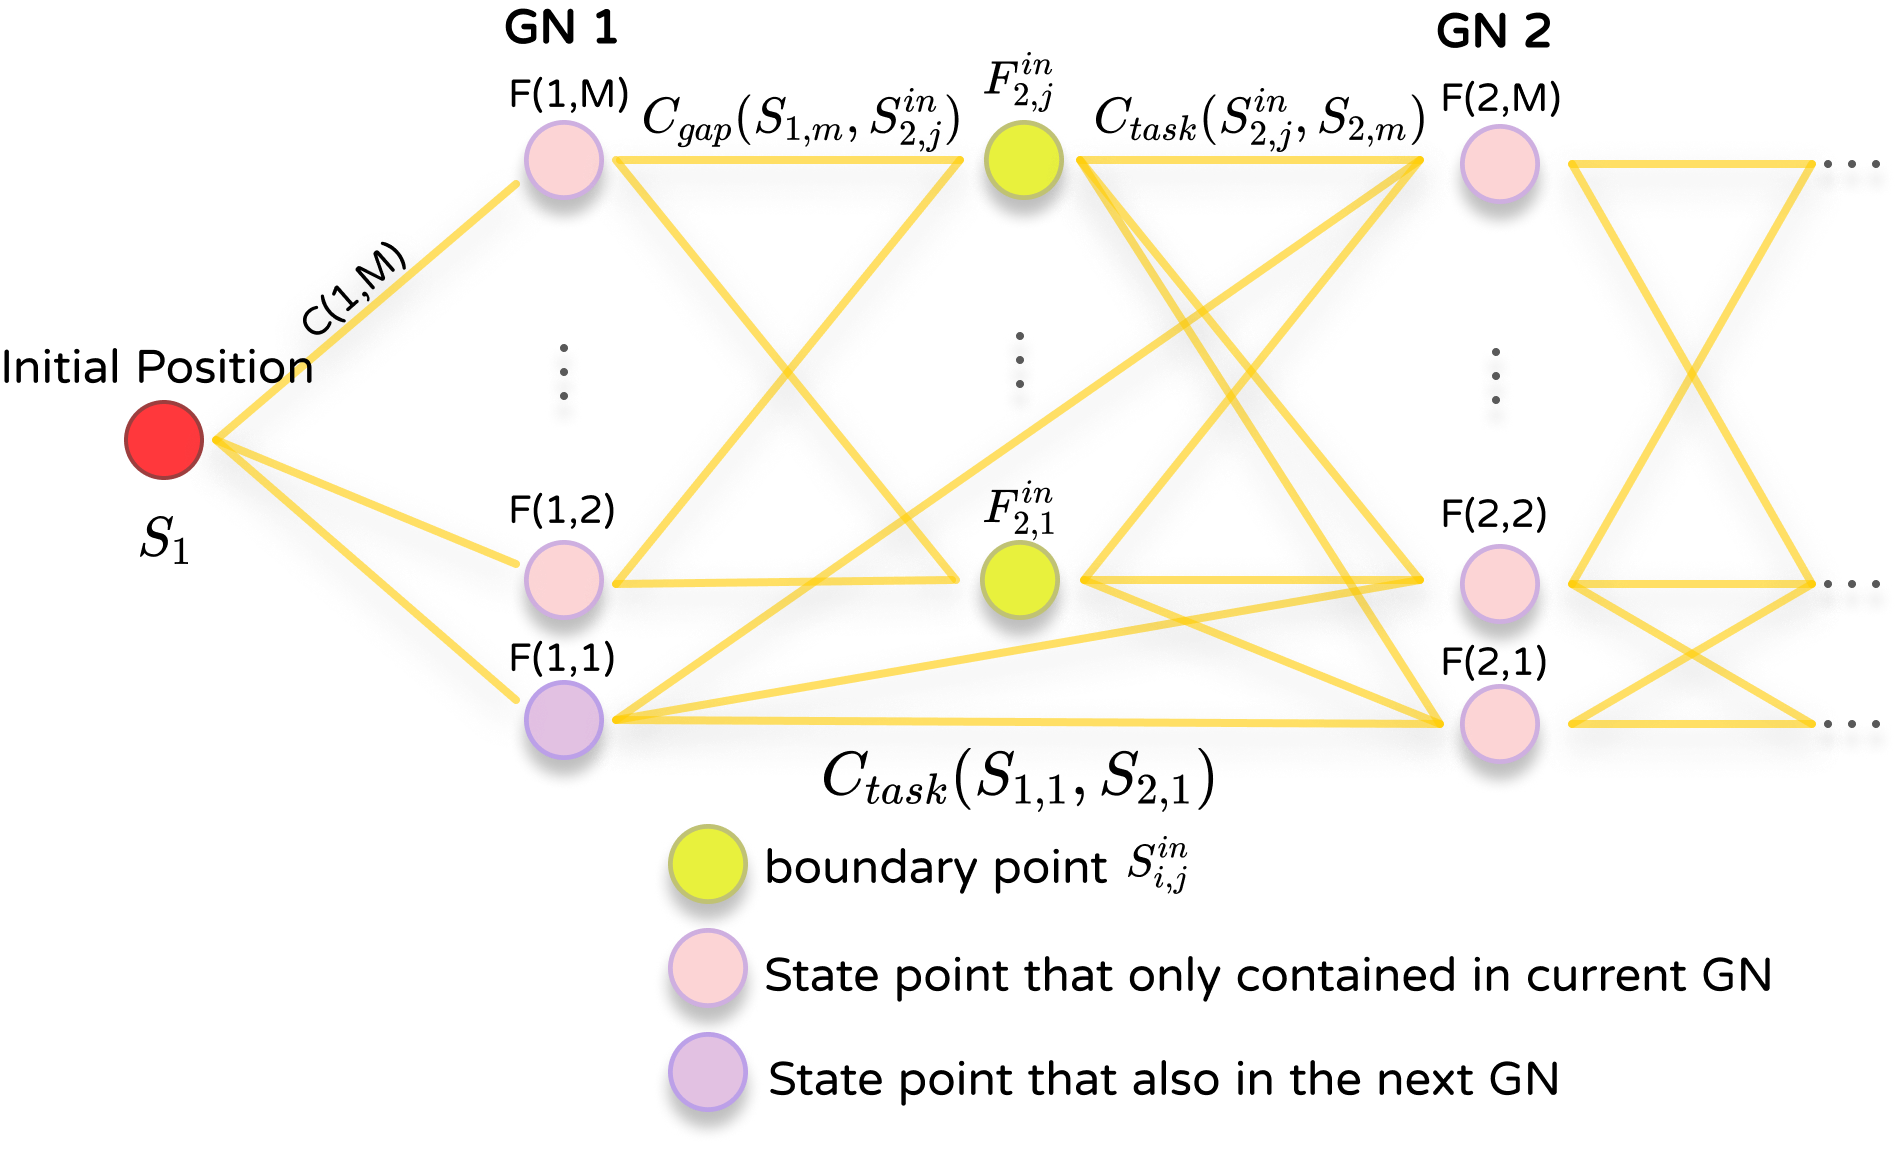
\includegraphics[width = 1 \linewidth]{figures/global-algorithm-flowchart.png}
    \caption{ Stage-wise state-transition structure of the proposed ORE dynamic programming algorithm. The mission is decomposed into per-GN stages: within the communication region of each $GN_i$, discrete exit-state points (pink: contained only in the current GN; purple: already inside the next GN's coverage) and boundary entry state points $S^{in}_{i,j}$ (green) are enumerated. Each inter-stage transition cost is decomposed into a gap-segment cost $C_{gap}$ and a task-segment cost $C_{task}$. Starting from the initial state $S_1$, the algorithm recursively accumulates the minimum reached energy $F_{i,m}$ over all feasible predecessor states, turning the continuous JHVSO problem into a shortest-path search.}
   \label{fig:rough_process}
\end{figure}

In this section, we present the algorithmic framework designed to address the joint speed optimize problem.
Specifically, we delineate the calculation of the local transition cost between consecutive state points, formulate the recursive solution for the Optimal Reached Energy (ORE) sub-problem, and establish the theoretical optimality of the global scheduling algorithm.
The candidate state sets $GN_i$ are pre-filtered by the altitude bounds $h_{\min}\le h\le h_{\max}$ during state-space construction, so the dynamic program operates on altitude-feasible states only.

\subsection{Calculation for Local Transition Cost}

Fig.~(\ref{fig:rough_process}) described how algorithm calculating through ground nodes.
The proposed algorithm operates stage-by-stage across consecutive ground nodes.
Initiating from the initial state $S_0$, the algorithm evaluates the ORE sub-problem for $GN_1$ to determine $F_{1,m}$ for all candidate states $m \in GN_1$.
This is achieved by compounding the initial condition with the transition cost from $S_0$ to each state point associated with $GN_1$.
Once the optimal values for the first stage are derived, they serve as the foundational prefix costs for the subsequent stage.
By recursively integrating these state costs with the localized transition costs between $GN_1$ and $GN_2$, the search space is advanced sequentially.
Given its pivotal role as the building block of the recursive formulation, the accurate calculation of the local transition cost is paramount.

\begin{figure}[]
  \centering
   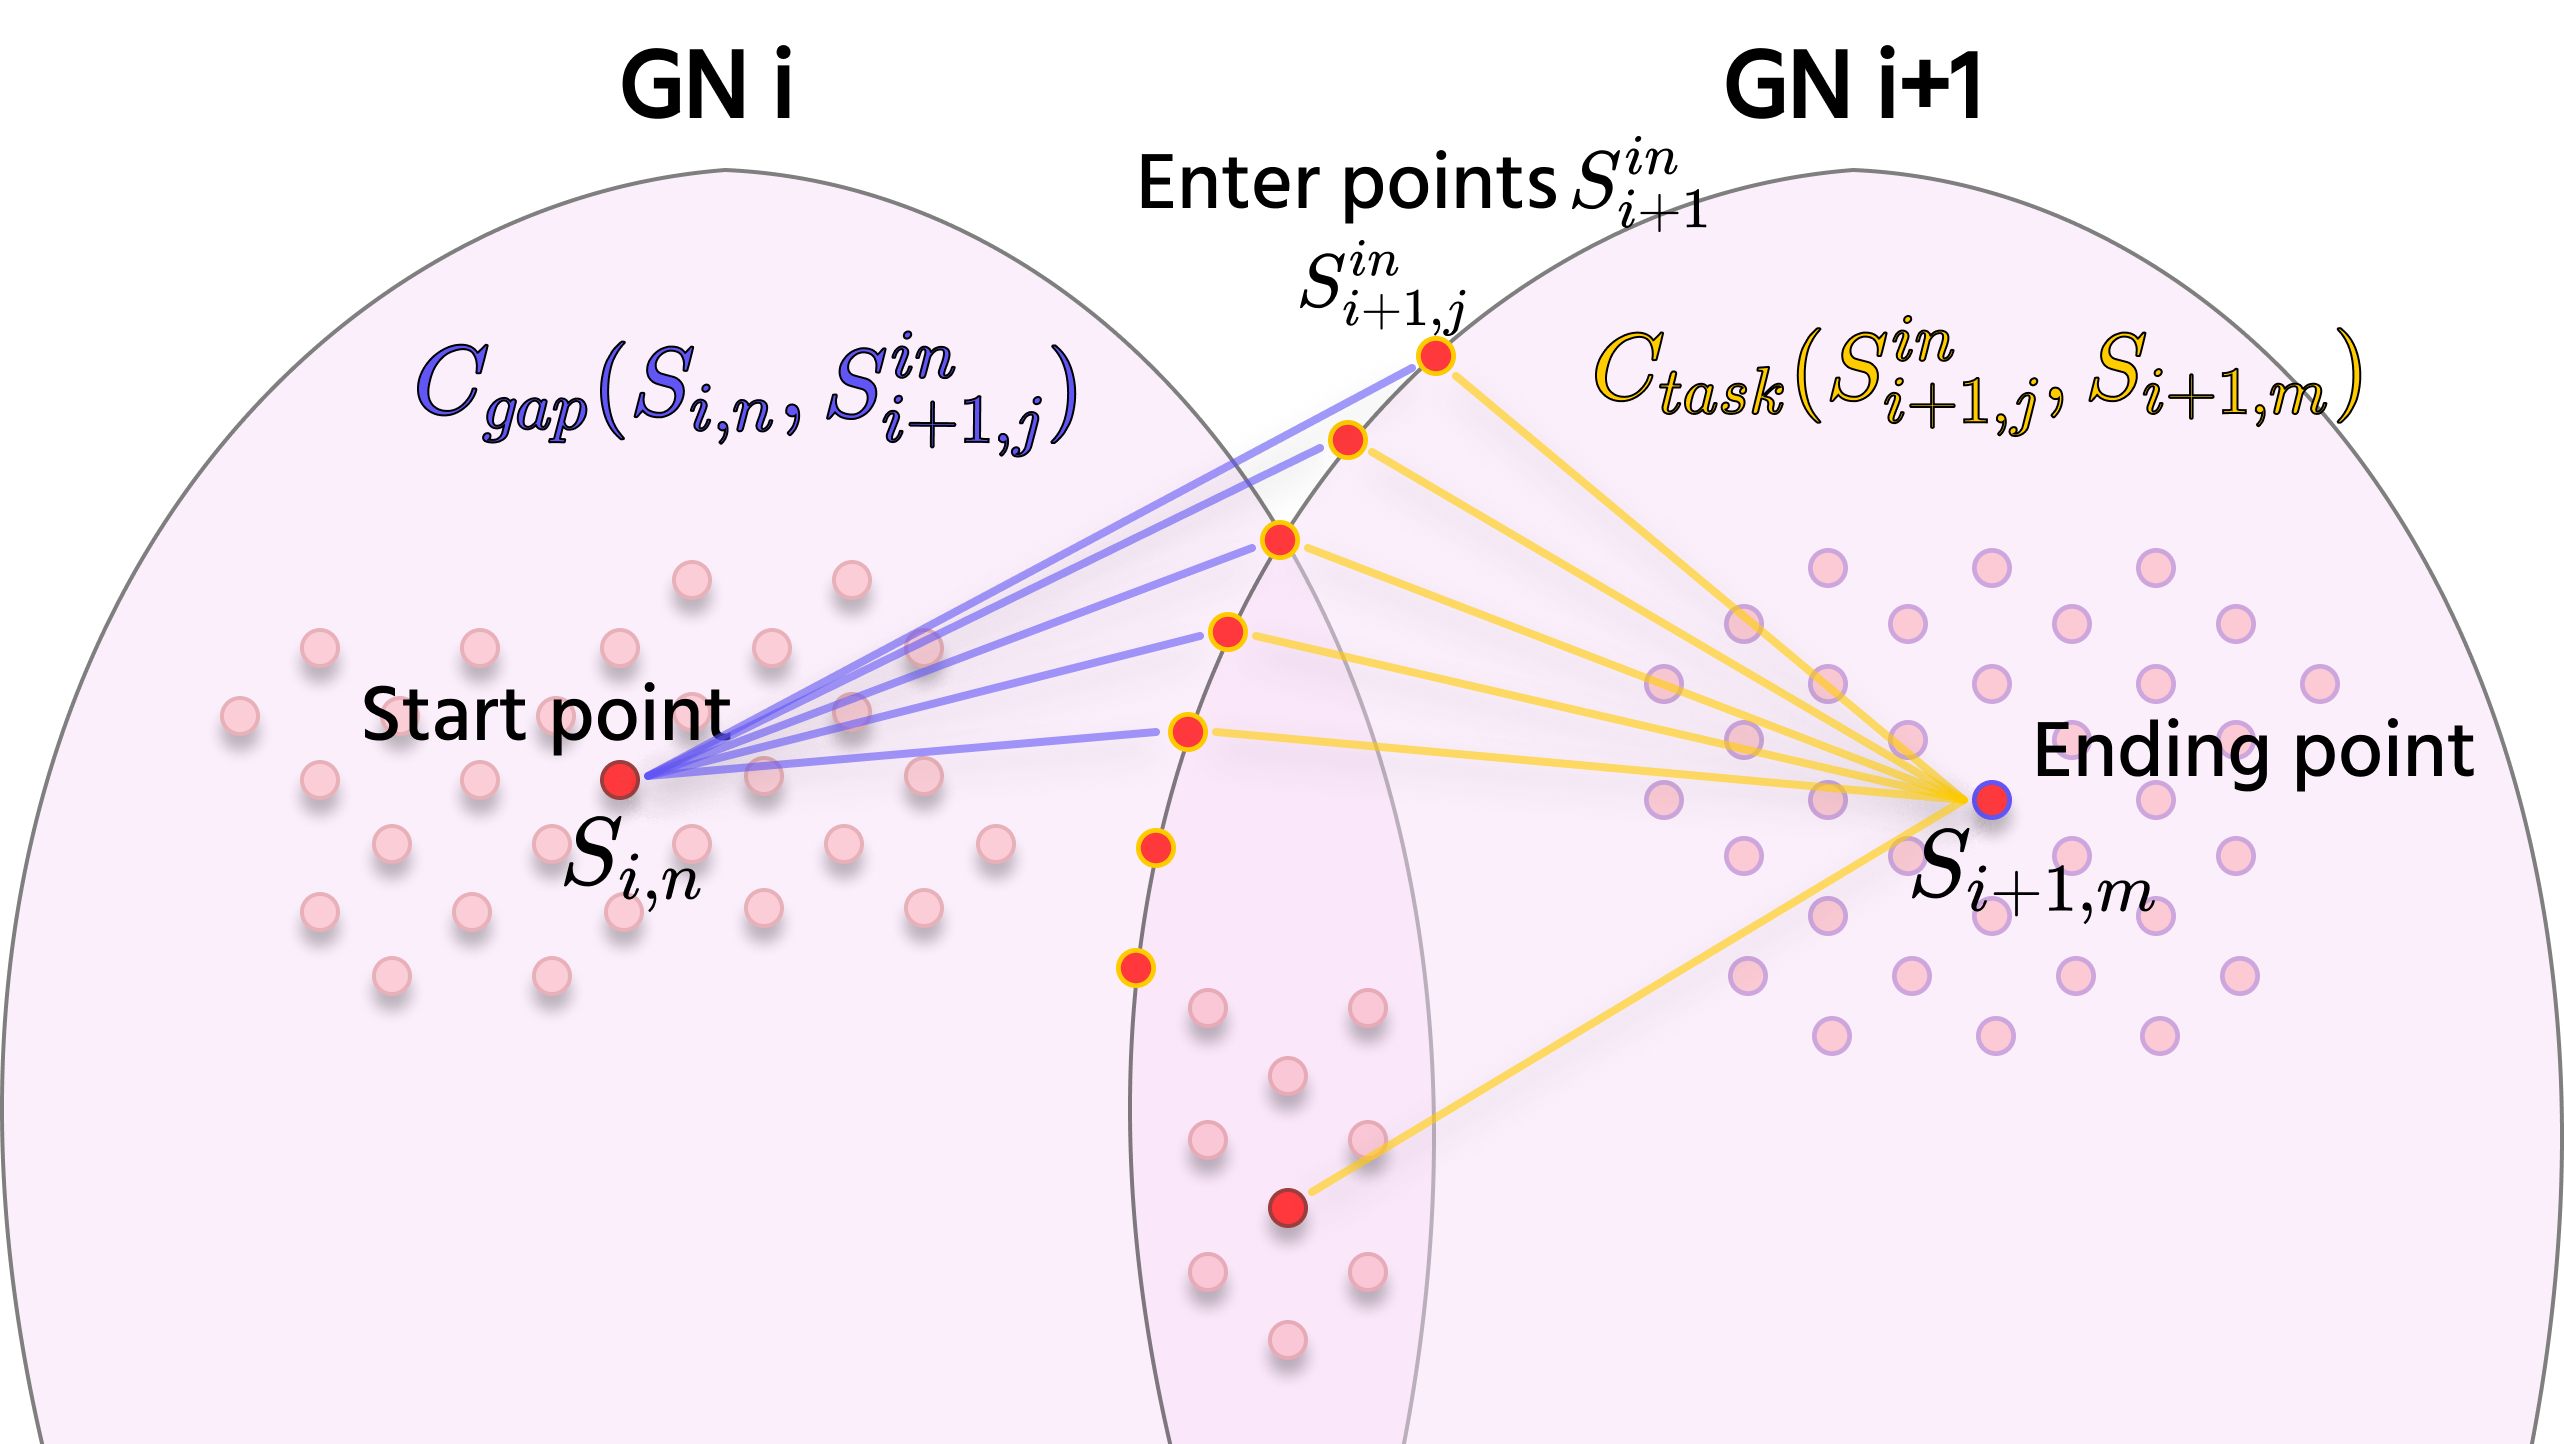
\includegraphics[width = 1\linewidth]{figures/transition-cost-case-1.png}
    \caption{Local transition cost between two state points $S_{i,n}$ (an exit state of $GN_i$) and $S_{i+1,m}$ (a target exit state in $GN_{i+1}$). When $S_{i,n}$ lies outside the coverage of $GN_{i+1}$, the transition is split at a boundary entry point $S^{in}_{i+1,j}$: a gap segment with cost $C_{gap}(S_{i,n}, S^{in}_{i+1,j})$, flown at the pitch-angle-dependent energy-optimal speed (Theorem~\ref{thm:optimal-range-speed}), followed by a task segment with cost $C_{task}(S^{in}_{i+1,j}, S_{i+1,m})$, flown at constant velocity that exactly fulfills the required collection duration $\tau_{i+1}$ (Theorem~\ref{thm:constant-speed}). The transition cost is the minimum compounded cost over all candidate entry points (Eq.~(\ref{equ:local_transition})).}
   \label{fig:transition-cost-case-1}
\end{figure}

Fig.~(\ref{fig:transition-cost-case-1}) show the way to evaluate the transition cost between exit state $S_{i,n}$ at stage $i$ and a target state  $S_{i+1,m}$ at stage $i+1$, the algorithm first evaluates their spatial alignment.
If the exit state already lies within the transmission coverage of the subsequent node $(S_{i,n} \in GN_{i+1})$, no gap cruising is required.
In this case, the transition cost is directly modelled as a straight-line flight spanning the distance $||S_{i,n},S_{i+1,m}||$ executed at a constant speed $v = ||S_{i,n},S_{i+1,m}||/\tau_{i+1}$, where $\tau_{i+1}$ represents the minimum required time for data collection duration.

Meanwhile, when the starting state resides outside the coverage of the next node $(S_{i,n} \notin GN_{i+1})$, the flight path between $S_{i,n}$ and $S_{Pi+1,m}$, must be partitioned into a gap segment and a task segment.
The configuration of the candidate trajectories is dictated by the entry states $S^{in}_{i+1,j}$ of $GN^{in}_{i+1}$ in \textit{Definition. \ref{def:state}}.
The algorithm evaluates all candidate transitions by linking the exit state $S_{i,n}$ to each entry point $S^{in}_{i+1,j}$ to compute the gap transition cost $C_{gap}(S_{i,n},S^{in}_{i+1,j})$.
To optimize this unconstrained cruise phase, the look-up function $LUT(\gamma)$ defined in Eq.~(\ref{equ:lut}) is utilized, which pre-computes the energy-per-meter optimum from the horizontal and vertical propulsion models across pitch angles, subject to the component-wise speed limits.

Following the gap segment, the task transition cost $C_{task}(S^{in}_{i+1,j},S_{i+1,m})$ is computed for the data collection phase within the communication range.
The total local transition cost between the two states is then determined by identifying the optimal boundary entry point that minimizes the compounded energy of both segments:

\[C(S_{i,n},S_{i+1,m}) = \min_{\forall S^{in}_{i+1,j}\in GN^{in}_{i+1}}(C_{gap}(S_{i,n},S^{in}_{i+1,j})\]
\[+C_{task}(S^{in}_{i+1,j},S_{i+1,m}))\]


\begin{algorithm}
    \caption{local transition cost calculation between two states}\label{alg:local_transition_cost}  
    \begin{algorithmic}[1]
        \Require $S_{i,n},S_{i+1,m},S^{in}_{i+1},\tau_{i+1}$
        \If{$S_{i,n}\in GN_{i+1}$}
            \State $C(S_{i,n},S_{i+1,m})=p \left(\frac{||S_{i,n},S_{i+1,m}||}{\tau_{i+1}}\right)\times \tau_{i+1}$
        \Else
            \State //$\gamma(S_{i,n},S^{in}_{i+1,j})$ means the angle of pitch between two states
            \For{$\forall S^{in}_{i+1,j} \in GN^{in}_{i+1}$}
                \State $C_{gap}(S_{i,n},S^{in}_{i+1,j}) = LUT(\gamma(S_{i,n},S^{in}_{i+1,j}))\times ||S_{i,n},S^{in}_{i+1,j}||$
                \State $C_{task}(S_{i,n},S^{in}_{i+1,j}) = P \left(\frac{||S^{in}_{i+1,j},ƒS_{i+1,m}||}{\tau_{i+1}}\right)\times \tau_{i+1}$
                \State $C_{S^{in}_{i+1,j}} = C_{gap}(S_{i,n},S^{in}_{i+1,j})+ C_{task}(S_{i,n},S^{in}_{i+1,j})$
            \EndFor
            \State $$C(S_{i,n},S_{i+1,m}) = \min_{\forall S^{in}_{i+1,j}\in GN^{in}_{i+1}}(E_{S^{in}_{i+1,j}})$$
        \EndIf
    \end{algorithmic}
\end{algorithm}

\begin{lemma}
    For any given pair of state points $S_{i,n}$ and $S_{i+1,m}$ at consecutive stages $i$ and $i+1$, the local transition cost $C(S_{i,n}, S_{i+1,m})$ is the theoretical minimum energy path under the defined constraints.
\end{lemma}

\begin{proof}
    The transition cost calculation is bifurcated based on the spatial relationship between the exit state $S_{i,n}$ and the transmission range of the target ground node ($GN_{i+1}$).

    \begin{enumerate}[a)]
    \item In-Range Transition ($S_{i,n} \in GN_{i+1}$)

    When the exit state $S_{i,n}$ resides within the transmission coverage of the target ground node, the transition is categorized as pure task segment.
    The transition cost $C_{task}$ is computed based on the displacement (distance and altitude) between $S_{i,n}$ and $S_{i+1,m}$ over the required data collection duration $\tau_{i+1}$.
    As established in \textit{Theorem. \ref{thm:constant-speed}}, for any given horizontal distance and altitude differential, maintaining a constant velocity over mission required duration $\tau$ is the most energy-efficient flight strategy.
    Thus, the transition cost in this scenario is theoretical optimal.
    \item Out-of-Range Transition ($S_{i,n} \notin GN_{i+1}$)

    For scenarios where the starting state lies outside the target transmission range, the trajectory is partitioned into a "gap segment" and a "task segment" via the boundary entry points $S_{i+1,j}^{in} \in GN^{in}_{i+1}$.
    The validity of this decomposition relies on two fundamental properties:
        \begin{itemize}
        \item Non-aftereffect Property: The UAV’s flight energy consumption model is solely a function of instantaneous velocity, implying that propulsion energy is independent of the UAV's velocity history.
        Furthermore, the time constraint $\tau_{i+1}$ is strictly imposed on the task segment, leaving the gap segment unconstrained in time.
        Consequently, the transition process satisfies the non-aftereffect property, allowing the optimization of the two segments to be decoupled.
        \item Optimality: The optimality of the task segment is guaranteed by \textit{Theorem. \ref{thm:constant-speed}}.
        For the gap segment, \textit{Theorem. \ref{thm:optimal-range-speed}} demonstrates that the energy-optimal strategy is to maintain a constant speed that minimizes energy consumption per unit distance.
        \end{itemize}  
    By systematically evaluating all feasible entry points on the transmission boundary and integrating the independently optimized costs for the gap and task segments, the resulting transition cost $C(S_{i,n}, S_{i+1,m})$ represents the theoretical optimum for the stage transition.
    \qed
    \end{enumerate}  
\end{proof}

\subsection{Solution for ORE and JHVSO Problem}

Before presenting the recursive solution, we first address a computational bottleneck inherent in the direct application of \textit{Algorithm. \ref{alg:local_transition_cost}}.
Suppose the preceding node $GN_i$ and current node $GN_{i+1}$ are discretized into $m$ and $n$ candidate states, respectively, and the transmission boundary of $GN_{i+1}$ is sampled by $j$ entry points.
Evaluating the ORE recurrence Eq.~(\ref{equ:ore_1}) by computing the local transition cost $C(S_{i,n},S_{i+1,m})$ independently for every state pair requires, for each of the $m\times n$  pairs, an enumeration of all $j$  entry points to identify the optimal compounded energy of the Gap and Task segments, resulting in a per-stage complexity of $O(m\times j \times n)$.

This overhead can be eliminated through a decoupled evaluation order.
Observe that in the compounded transition cost of Eq.~(\ref{equ:ore_1}), the Gap-segment term $C_{gap}(S_{i,n},S^{in}_{i+1,j})$ is independent of the target state $S_{i+1,m}$, the Task-segment term $C_{task}(S^{in}_{i+1,j},S_{i+1,m})$ is independent of the exit state $S_{i,n}$, and the prefix energy $F_{i,n}$ is independent of the entry point.
Substituting Eq.~(\ref{equ:local_transition}) into the ORE recurrence and rearranging the two minimizations therefore yields
\begin{align}\label{equ}
    &F_{i+1,m} = \min_{\forall S^{in}_{i+1,j}}(\min_{\forall S_{i,n} \notin GN_{i+1}}(F_{i,n} + C_{gap}(S_{i,n},S^{in}_{i+1,j}) + 
    \nonumber
    \\ &C_{task}(S^{in}_{i+1,j},S_{i+1,m})))
\end{align}

The inner minimization is precisely the ORE value of the entry state (Definition. \ref{def:ORE}),

\begin{equation}
F^{in}_{i+1,j} = \min_{\substack{S_{i,n} \in GN_i \\ S_{i,n} \notin GN_{i+1}}} \big\{ F_{i,n} + C_{gap}(S_{i,n}, S^{in}_{i+1,j}) \big\},
\label{equ:fin}
\end{equation}
i.e., the minimum energy of completing the first $i$ tasks and cruising to the boundary point $S^{in}_{i+1,j}$.
It depends only on the exit states and the entry points, and is therefore computed exactly once for each exit-state--entry-point pair and reused by all $n$ target states.
The outer minimization then projects the entry costs onto the exit states through the task segments,
\[
F_{i+1,m} = \min\Big\{ \underbrace{\min_{j} \big\{ F^{in}_{i+1,j}+ C_{task}(S^{in}_{i+1,j}, S_{i+1,m}) \big\}}_{\text{via boundary entry}},\;
\]
\[
 \underbrace{\min_{S_{i,n} \in GN_i , S_{i,n} \in GN_{i+1}} \big\{ F_{i,n} + C_{task}(S_{i,n}, S_{i+1,m}) \big\}}_{\text{overlap, direct task}} \Big\}
\]
The evaluation is thus reorganized into two decoupled phases with complexities $O(m \times j)$ and $O(j \times n)$, reducing the per-stage overhead from $O(m \times j \times n)$ to $O(m \times j + j\times n)$.
Transitions originating from overlapping states that already reside within the coverage of $GN_{i+1}$ involve no entry points and are evaluated directly through the Task segment, which is unaffected by this restructuring.
Crucially, the rearrangement is an exact algebraic restructuring rather than an approximation: every candidate trajectory composed of an exit state, an entry point, and a target state is still examined, and each is examined exactly once, so the resulting ORE values are identical to those of the pairwise evaluation.
The validity of compounding the prefix energy with the Gap cost at a boundary entry point—without regard to the target state that follows—is precisely the non-aftereffect property established in \textit{Theorem. \ref{thm:aftereffect}}, applied here with the entry point acting as the intermediate state.
We now formalize this two-phase evaluation in the ORE algorithm.

With the local transition cost formalized, we extend the framework to solve the Optimal Reached Energy (ORE) sub-problem recursively.
The ORE sub-problem at stage $i+1$, denoted as $F_{i+1,m}$, aims to find the energy-minimal trajectory that completes data collection for the first $i+1$ ground nodes, terminating precisely at the state $S_{i+1,m}$.
This framework systematically leverages the optimized state values $F_{i,n}$, computed from the preceding stage $i$.

\begin{figure}[]
  \centering
   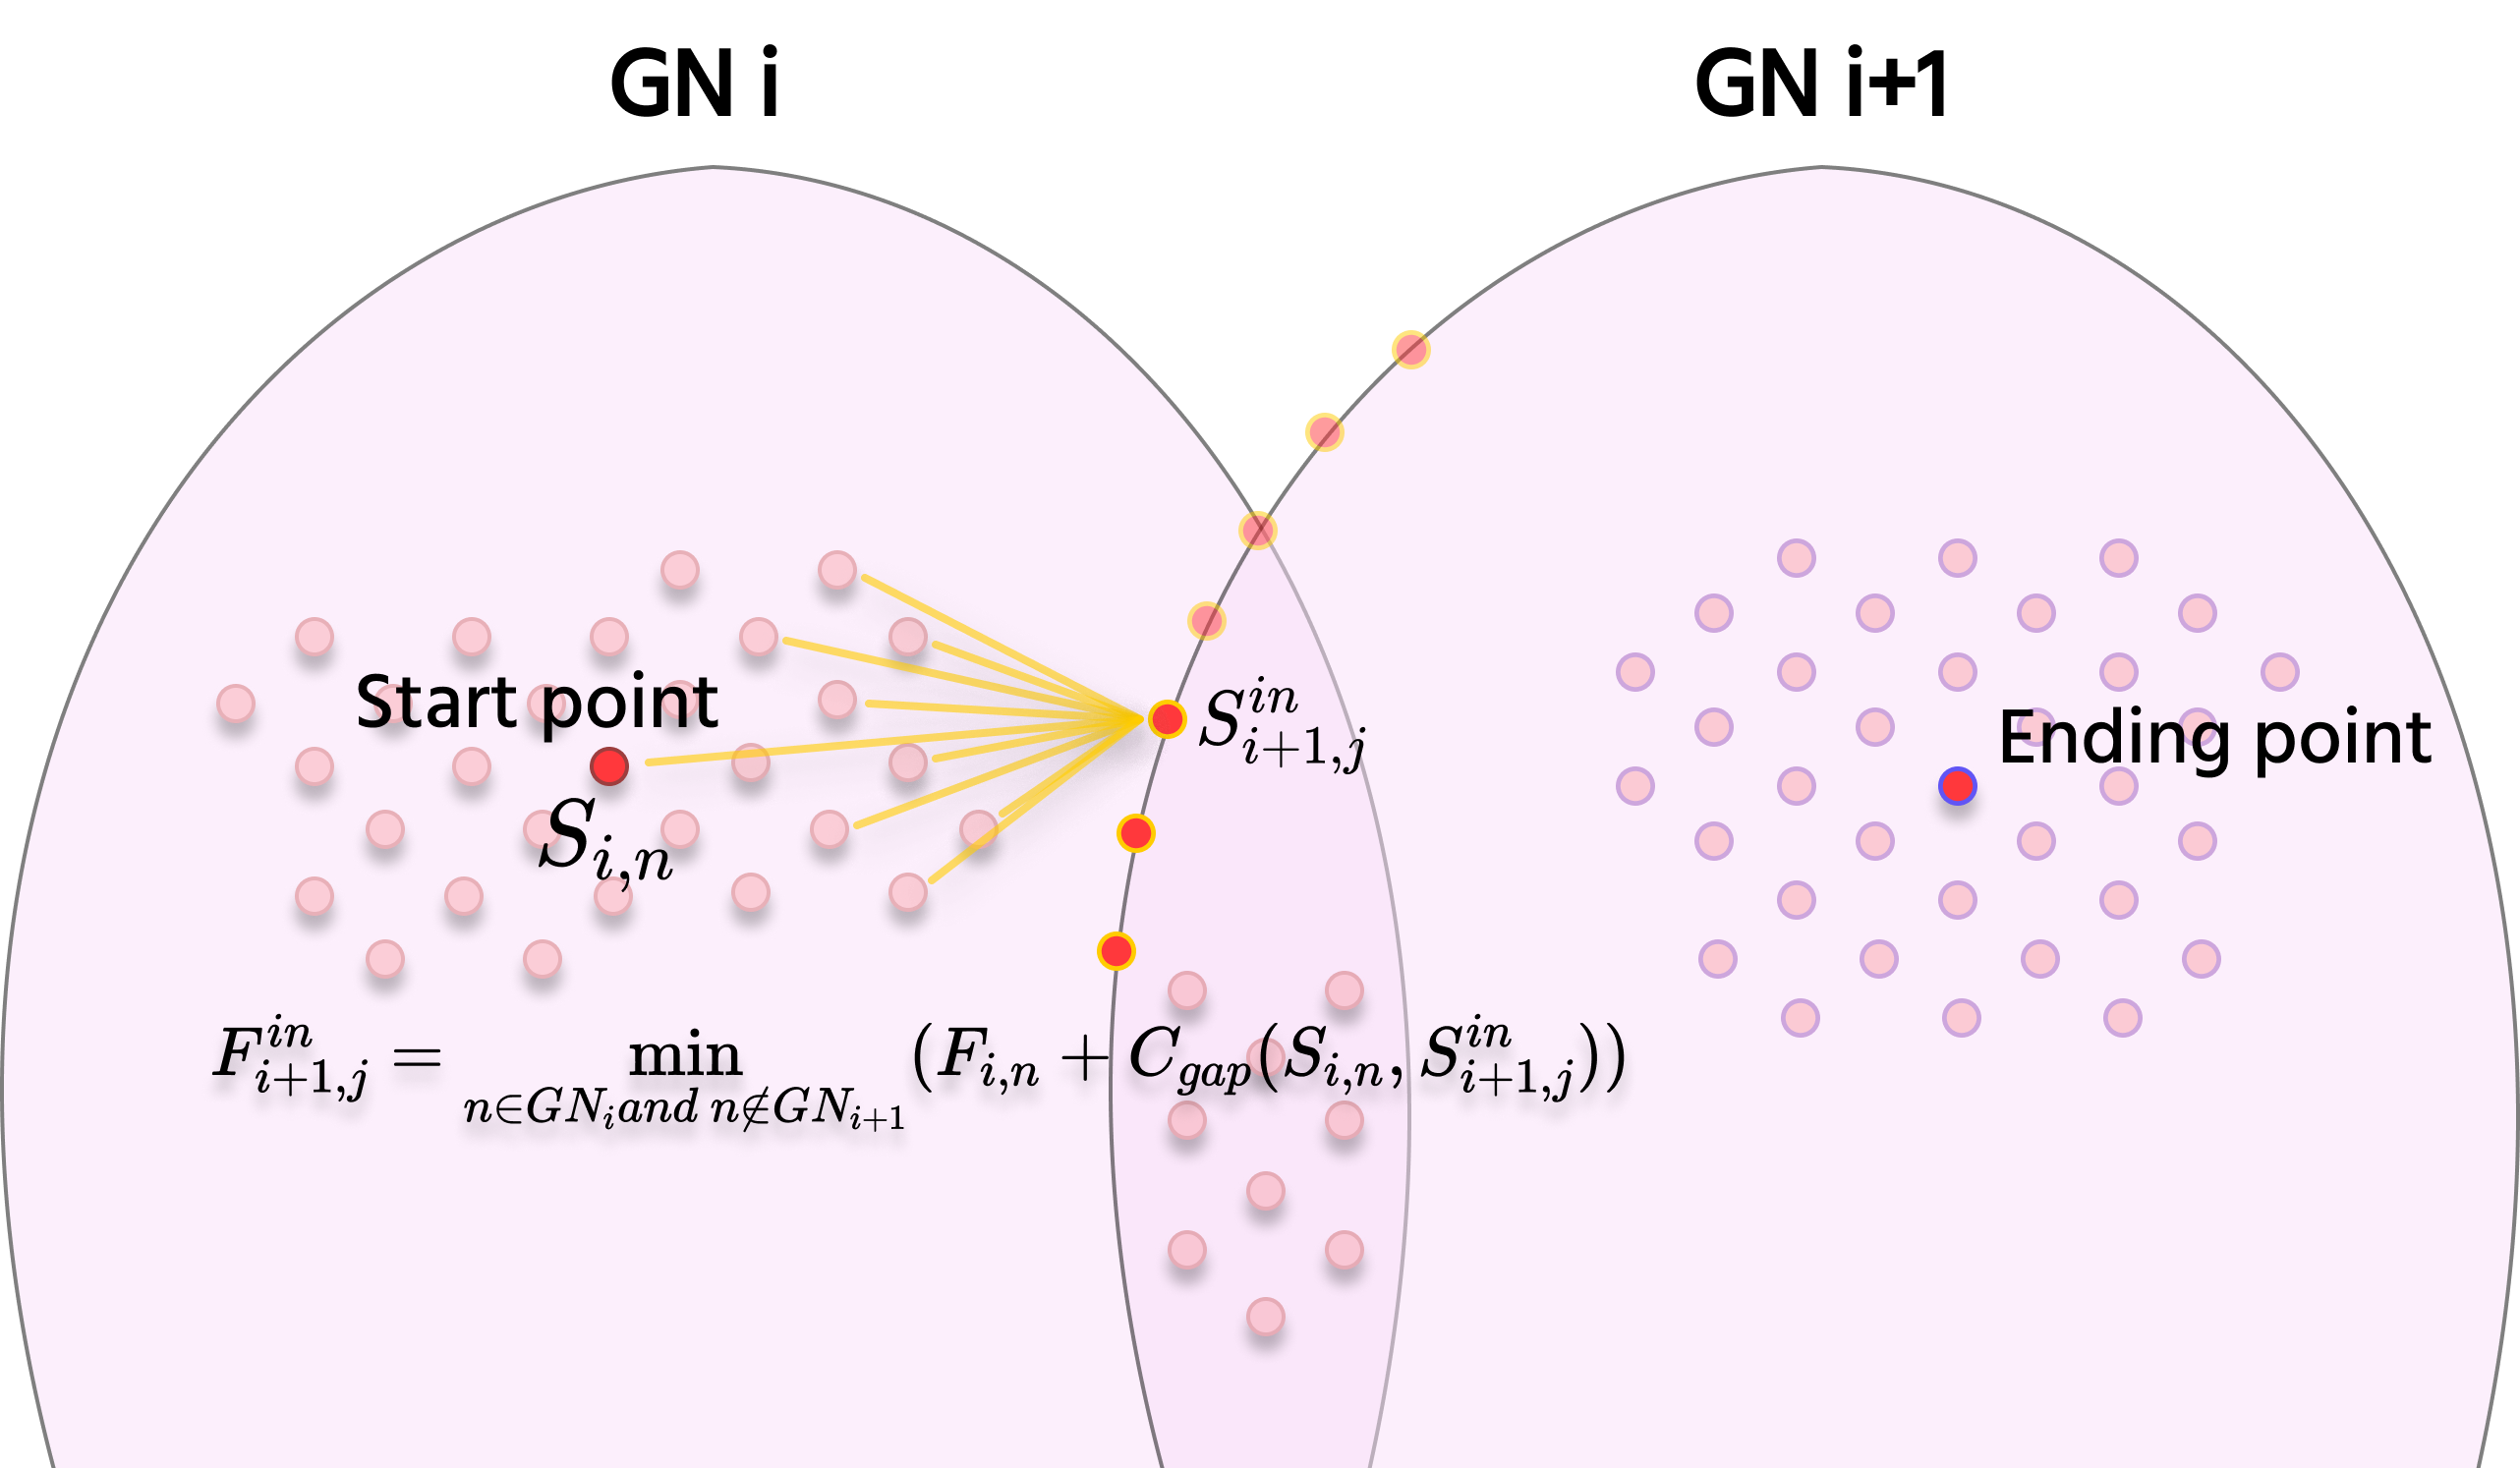
\includegraphics[width = 1\linewidth]{figures/transition-cost-case-2.png}
    \caption{ The energy cost of the mid-stage state point $F^{in}_{i+1}$ is computed by considering all state points from the previous stage that outside the communication range of $GN_{i+1}$.
    For each feasible predecessor state, the accumulated energy cost is added to the gap cost from that state to $S^{in}_{i+1}$.
    The minimum of these total costs is then taken as the energy cost of $F^{in}_{i+1}$}\label{fig:to_mid_stage}
\end{figure}

The calculation filters all candidate states from the previous stage that do not overlap with the current node's range, satisfying $S_{i,n}\notin GN_{i+1}$.
By mapping the gap costs  $C_{gap}$ from these disjoint states to the boundary entry points, the intermediate cost $F^{in}_{i+1,j}$ is minimized over the sum of the accumulated prefix energy and the cruise energy.

Once the optimal intermediate energy $F^{in}_{i+1,j}$ to reach the entry boundaries is established, the task costs $C_{task}(S^{in}_{i+1,j},$ $S_{i+1,m})$ are incorporated to project the path to the final state $S_{i+1,m}$, yielding a candidate value $\alpha$.
Simultaneously, the algorithm accounts for overlapping cases where prior states already reside within the transmission range of the current node $(S_{i,n} \in GN_{i} \cap GN_{i+1})$.
For these overlapping states, the task cost $C_{task}(S_{i,n},S_{i+1,m})$ is computed directly without a gap phase, yielding a candidate value $\beta$.
The ultimate ORE value $F_{i+1,m}$ is then determined by selecting the absolute minimum between these two operational pathways.


\begin{algorithm}
    \caption{ORE}\label{alg:ORE}  
    \begin{algorithmic}[1]
        \Require $GN_i, GN_{i+1},F_i,S^{in}_{i+1},\tau_{i+1}$
        \For{$S^{in}_{i+1,j} \in S^{in}_{i+1}$}
            \For{$\forall S_{i,n}\in GN_{i}\  and\  S_{i,n}\notin GN_{i+1}$}
                \State $F^{in}_{i+1,j} = \min(F_{i,n}+C_{gap}(S_{i,n},S^{in}_{i+1,j}))$
            \EndFor
        \EndFor
        \For{$S^{in}_{i+1,j} \in S^{in}_{i+1}$}
            \State $\alpha = \min (F^{in}_{i+1,j} + C_{task}(S^{in}_{i+1,j},S_{i+1,m}))$
        \EndFor
        \For{$\forall S_{i,n}\in GN_{i}\  and\  S_{i,n}\in GN_{i+1}$}
            \State $\beta = \min (F_{i,n} + C_{task}(S_{i,n},S_{i+1,m}))$
        \EndFor
        \State $F_{i+1,m} = min(\alpha,\beta)$
    \end{algorithmic}
\end{algorithm}
Once the ORE values are resolved for all stages, the global Joint horizontal-vertical speed optimization (JHVSO) problem can be straightforwardly solved.
The global energy-optimal trajectory encompassing all N ground nodes is obtained by identifying the minimum cost among all feasible terminal states at the final stage, expressed as $\min(F_N)$.

\begin{algorithm}
    \caption{JHVSO}\label{alg:JHVSO}  
    \begin{algorithmic}[1]
        \Require $S_0,GN_{1 \dots N},\tau_{1\dots N},h_f$
        \For{$GN_i \in GN_{1 \dots N}$}
            \For{$S_{i,m} \in GN_{i}$}
                \State $F_{i,m} = ORE(F_{i-1},S_{i,m})$
            \EndFor
        \EndFor
        \State $JHVSO = \min_{h=h_f}(F_{N})$
    \end{algorithmic}
\end{algorithm}


\begin{figure}[]
  \centering
   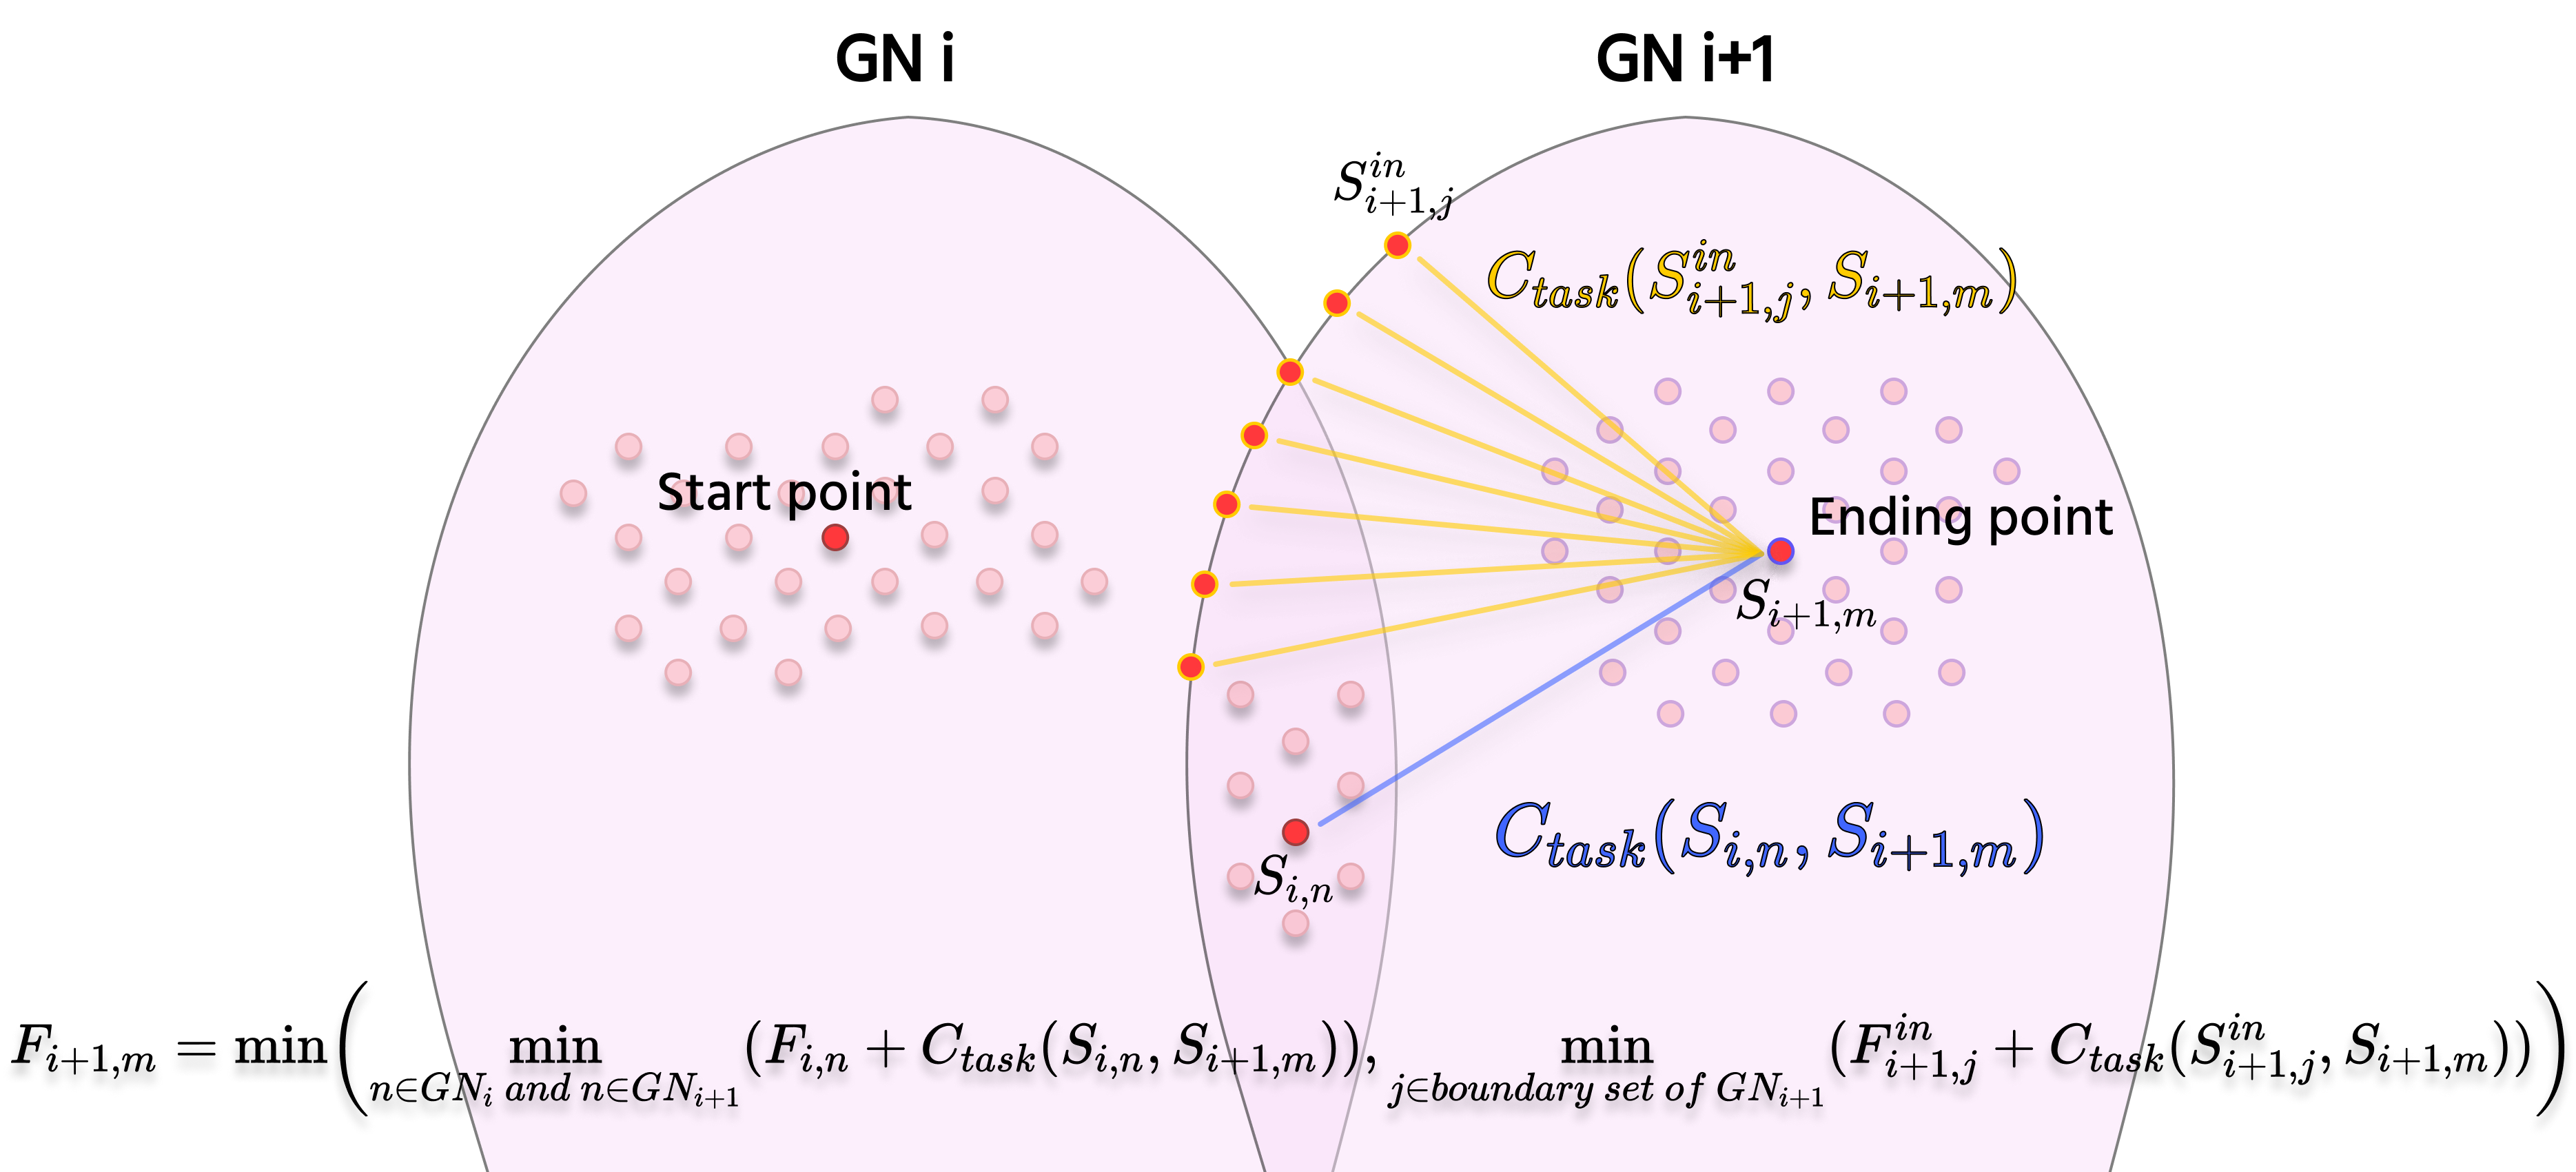
\includegraphics[width = 1\linewidth]{figures/transition-cost-case-3.png}
    \caption{The energy cost of $S_{i+1,m}$ is obtained by evaluation all state points from the previous stage that are within the communication range of the current ground node $S_{i,n} \in GN_i\&GN_{i+1}$ and the mid-stage state points $S^{in}_{i+1}$ .
    For each feasible predecessor state, the corresponding task cost is added to its accumulated energy cost.
    The minimum resulting cost is assigned as the energy cost of $S_{i+1,m}$}\label{fig:from_mid_stage}
\end{figure}

\begin{theorem}
    For any stage $i \in \{1, 2, \dots, N\}$ and any discrete state $S_{i,m} \in GN_{i}$, the cumulative minimum energy consumption $F_{i,m}$ calculated by the proposed ORE algorithm is exactly equal to the theoretical global minimum energy consumption $G(S_{i,m})$, which means:
    $$F(S_{i,m}) = G(S_{i,m}), \quad \forall S_{i,m} \in GN_i, i \in {1, 2, \dots, N}$$
\end{theorem}


\begin{proof}
    The cumulative minimum energy consumption $F_{i,m}$ for state $S_{i,m}$ is calculated by finding the trajectory with minimum energy consumption from all possible states of previous stage.

$$F_{i,m} = \min_{\forall S_{i-1,n} \in GN_{i-1}} \{F_{i-1,n} + C(S_{i-1,n},S_{i,m})\}$$

The transition cost from these possible states to the target states has no aftereffect, as we have proved in \textit{Theorem.\ref{thm:aftereffect}}.
So we can using the principle of mathematical induction on the stage index $i$.

The induction runs over the stage boundaries, i.e., the exit states.
Within each stage, the value of every entry state is obtained from the preceding exit states through Eq.~(\ref{equ:fin}), whose optimality follows from the same non-aftereffect argument applied with the entry point as the intermediate state (\textit{Theorem.\ref{thm:aftereffect}}); hence it suffices to establish $F(S_{i,m}) = G(S_{i,m})$ at the exit states.

\textit{Base Case ($i = 1$):} At the beginning of the mission, the UAV departs from the unique initial deployment position $S_0$.
To reach any target state $S_{1,m} \in GN_1$ at the end of the first stage, there is no historical trajectory or prior decision path.
Therefore, the theoretical global minimum energy $G(S_{1,m})$ consists uniquely of the single-step transition from $S_0$ to $S_{1,m}, \forall m\in GN_1 $, which can be expressed as $G(S_{1,m}) = C(S_0, S_{1,m})$.
Since the local transition cost has been proven to be optimal above, it follows that $F(S_{1,m}) = G(S_{1,m})$ holds strictly for all $S_{1,m} \in GN_1$.

\textit{Inductive Hypothesis:} Assume that the theorem holds true for stage $i-1$.
That is, for any discrete state $S_{i-1,n}$ within the state space $GN_{i-1}$, the algorithmic cumulative cost satisfies the following condition:

$$F(S_{i-1,n}) = G(S_{i-1,n}), \quad \forall S_{i-1,n} \in GN_{i-1}$$

\textit{Inductive Step:} We now evaluate the optimality of the algorithm at stage $i$ .
Consider an arbitrary state $S_{i,m} \in GN_i$.
Due to the spatial and temporal continuity of the flight trajectory, any globally optimal path reaching $S_{i,m}$ must pass through a specific boundary state at the preceding stage $GN_{i-1}$.
Therefore, the theoretical absolute minimum energy $G(S_i,n)$ can be mathematically expanded into a two-stage optimization form:

% \begin{align}\label{equ}
%     &G(S_{i,m}) =  \min_{\forall S_{i-1,n} \in GN_{i-1}}  \{G(S_{i-1,n}) +
%     \nonumber
%     \\ & \textit{Theoretical transition cost  from } S_{i-1,n} \textit{ to } S_{i,m} \}
%     \nonumber
% \end{align}

$$G(S_{i,m}) = \min_{\forall S_{i-1,n} \in GN_{i-1}} { \{G(S_{i-1,n}) + C^*( S_{i-1,n} , S_{i,m} )\}}$$

By invoking the non-aftereffect property established above, the transition cost from $S_{i-1,n}$ to $S_{i,m}$ is fully decoupled from the trajectory prior to stage $i-1$.
Furthermore, as demonstrated in Subsection 5.1, the local scheduling method guarantees that the calculated cost $C(S_{i-1,n}, S_{i,m})$ reaches the physical lower bound.
Consequently, the theoretical transition cost matches the algorithmic transition cost, which simplifies the equation to:


$$G(S_{i,m}) = \min_{\forall S_{i-1,n} \in GN_{i-1}} { \{G(S_{i-1,n}) +  C(S_{i-1,n} , S_{i,m})\} }$$


Next, we substitute the inductive hypothesis $G(S_{i-1,n}) = F(S_{i-1,n})$ into the optimization term, yielding:


$$G(S_{i,m}) = \min_{\forall S_{i-1,n} \in GN_{i-1}} { \{F(S_{i-1,n}) + C(S_{i-1,n}, S_{i,m})\} }$$


By the principle of mathematical induction, since the base case holds and the inductive step preserves this equality, the relation $F(S_{i,m}) = G(S_{i,m})$ is valid for all stages $i \in \{1, 2, \dots, N\}$.
This completes the proof.
\qed
\end{proof}

%%%%%%%%%%%%%%%%%%%%%%%%%%%%%%%%%%%%%%%%%%%%%%%%%%%%%%%%%%%%%%%%%%%%%%%%%%%%%%%%%%
%%%%%%%%%%%%%%%%%%%%%%%%%%%%%%%%%%%%%%%%%%%%%%%%%%%%%%%%%%%%%%%%%%%%%%%%%%%%%%%%%%
 
